\documentclass[12pt,letterpaper]{article}
\usepackage[letterpaper,left=0.62in,right=0.62in,top=0.75in,bottom=0.65in,headheight=14pt,headsep=0.17in,footskip=0.32in]{geometry}
\usepackage[T1]{fontenc}
\usepackage{lmodern}
\pdfmapfile{+lm.map}
\usepackage{tikz}
\usepackage{fancyhdr}
\definecolor{Rfill}{RGB}{251,227,225}
\definecolor{Bfill}{RGB}{223,235,251}
\definecolor{Yfill}{RGB}{255,247,203}
\pagestyle{fancy}
\fancyhf{}
\renewcommand{\headrulewidth}{0pt}
\renewcommand{\footrulewidth}{0pt}
\setlength{\parindent}{0pt}
\setlength{\parskip}{0pt}
\setlength{\emergencystretch}{2em}
\raggedbottom
\sffamily
\fancyhead[L]{\fontsize{10.5}{12}\selectfont Week 16 / Three-color triangles / Grades 2--3}
\fancyfoot[L]{\fontsize{9}{11}\selectfont Bellingham Math Circle / Week 16 / F16-23-v2}
\fancyfoot[R]{\fontsize{9}{11}\selectfont\thepage}
\begin{document}
\fontsize{12.5}{16.5}\selectfont
Write R, B, or Y on every empty dot. Keep the printed letters. Each outside side allows only the letters beside it. A little triangle has no lines inside.\par\vspace{0.23in}
\textbf{Problem 1:} Find a filling with as few little triangles containing R, B, and Y as you can. Find another filling with as many as you can.\par\vspace{0.16in}
\begin{center}
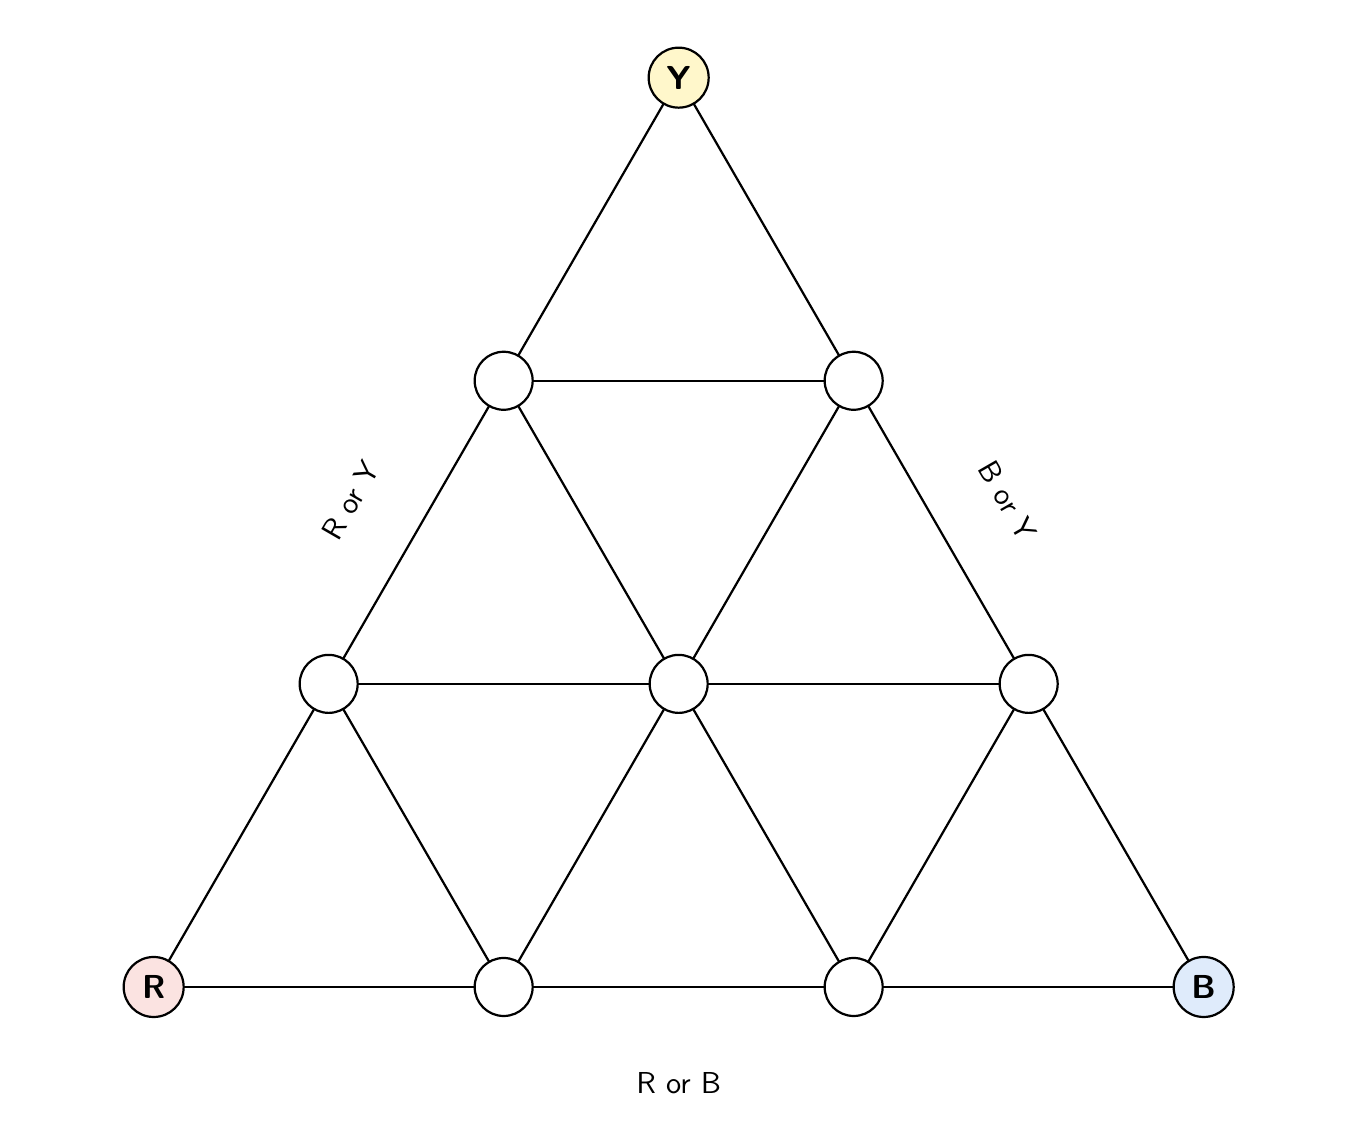
\begin{tikzpicture}[x=1in,y=1in,line cap=round,line join=round]
\path[use as bounding box] (-0.63,-0.64) rectangle (5.8800,4.7966);
\draw[line width=0.8pt] (0.0000,0.0000) -- (0.8750,1.5155);
\draw[line width=0.8pt] (0.0000,0.0000) -- (1.7500,0.0000);
\draw[line width=0.8pt] (0.8750,1.5155) -- (1.7500,3.0311);
\draw[line width=0.8pt] (0.8750,1.5155) -- (1.7500,0.0000);
\draw[line width=0.8pt] (0.8750,1.5155) -- (2.6250,1.5155);
\draw[line width=0.8pt] (1.7500,3.0311) -- (2.6250,4.5466);
\draw[line width=0.8pt] (1.7500,3.0311) -- (2.6250,1.5155);
\draw[line width=0.8pt] (1.7500,3.0311) -- (3.5000,3.0311);
\draw[line width=0.8pt] (2.6250,4.5466) -- (3.5000,3.0311);
\draw[line width=0.8pt] (1.7500,0.0000) -- (2.6250,1.5155);
\draw[line width=0.8pt] (1.7500,0.0000) -- (3.5000,0.0000);
\draw[line width=0.8pt] (2.6250,1.5155) -- (3.5000,3.0311);
\draw[line width=0.8pt] (2.6250,1.5155) -- (3.5000,0.0000);
\draw[line width=0.8pt] (2.6250,1.5155) -- (4.3750,1.5155);
\draw[line width=0.8pt] (3.5000,3.0311) -- (4.3750,1.5155);
\draw[line width=0.8pt] (3.5000,0.0000) -- (4.3750,1.5155);
\draw[line width=0.8pt] (3.5000,0.0000) -- (5.2500,0.0000);
\draw[line width=0.8pt] (4.3750,1.5155) -- (5.2500,0.0000);
\node[circle,draw,line width=0.8pt,fill=Rfill,minimum size=0.30in,inner sep=0pt,font=\sffamily\bfseries\fontsize{11.5}{12}\selectfont] at (0.0000,0.0000) {R};
\draw[line width=0.8pt,fill=white] (1.7500,0.0000) circle[radius=0.145in];
\draw[line width=0.8pt,fill=white] (3.5000,0.0000) circle[radius=0.145in];
\node[circle,draw,line width=0.8pt,fill=Bfill,minimum size=0.30in,inner sep=0pt,font=\sffamily\bfseries\fontsize{11.5}{12}\selectfont] at (5.2500,0.0000) {B};
\draw[line width=0.8pt,fill=white] (0.8750,1.5155) circle[radius=0.145in];
\draw[line width=0.8pt,fill=white] (2.6250,1.5155) circle[radius=0.145in];
\draw[line width=0.8pt,fill=white] (4.3750,1.5155) circle[radius=0.145in];
\draw[line width=0.8pt,fill=white] (1.7500,3.0311) circle[radius=0.145in];
\draw[line width=0.8pt,fill=white] (3.5000,3.0311) circle[radius=0.145in];
\node[circle,draw,line width=0.8pt,fill=Yfill,minimum size=0.30in,inner sep=0pt,font=\sffamily\bfseries\fontsize{11.5}{12}\selectfont] at (2.6250,4.5466) {Y};
\node[rotate=60,font=\sffamily\fontsize{11}{12}\selectfont] at (0.9825,2.4333) {R or Y};
\node[rotate=-60,font=\sffamily\fontsize{11}{12}\selectfont] at (4.2675,2.4333) {B or Y};
\node[font=\sffamily\fontsize{11}{12}\selectfont] at (2.6250,-0.48) {R or B};
\end{tikzpicture}
\end{center}
\newpage
\textbf{Problem 1:} Find a filling with as few little triangles containing R, B, and Y as you can. Find another filling with as many as you can.\par\vspace{0.16in}
\begin{center}
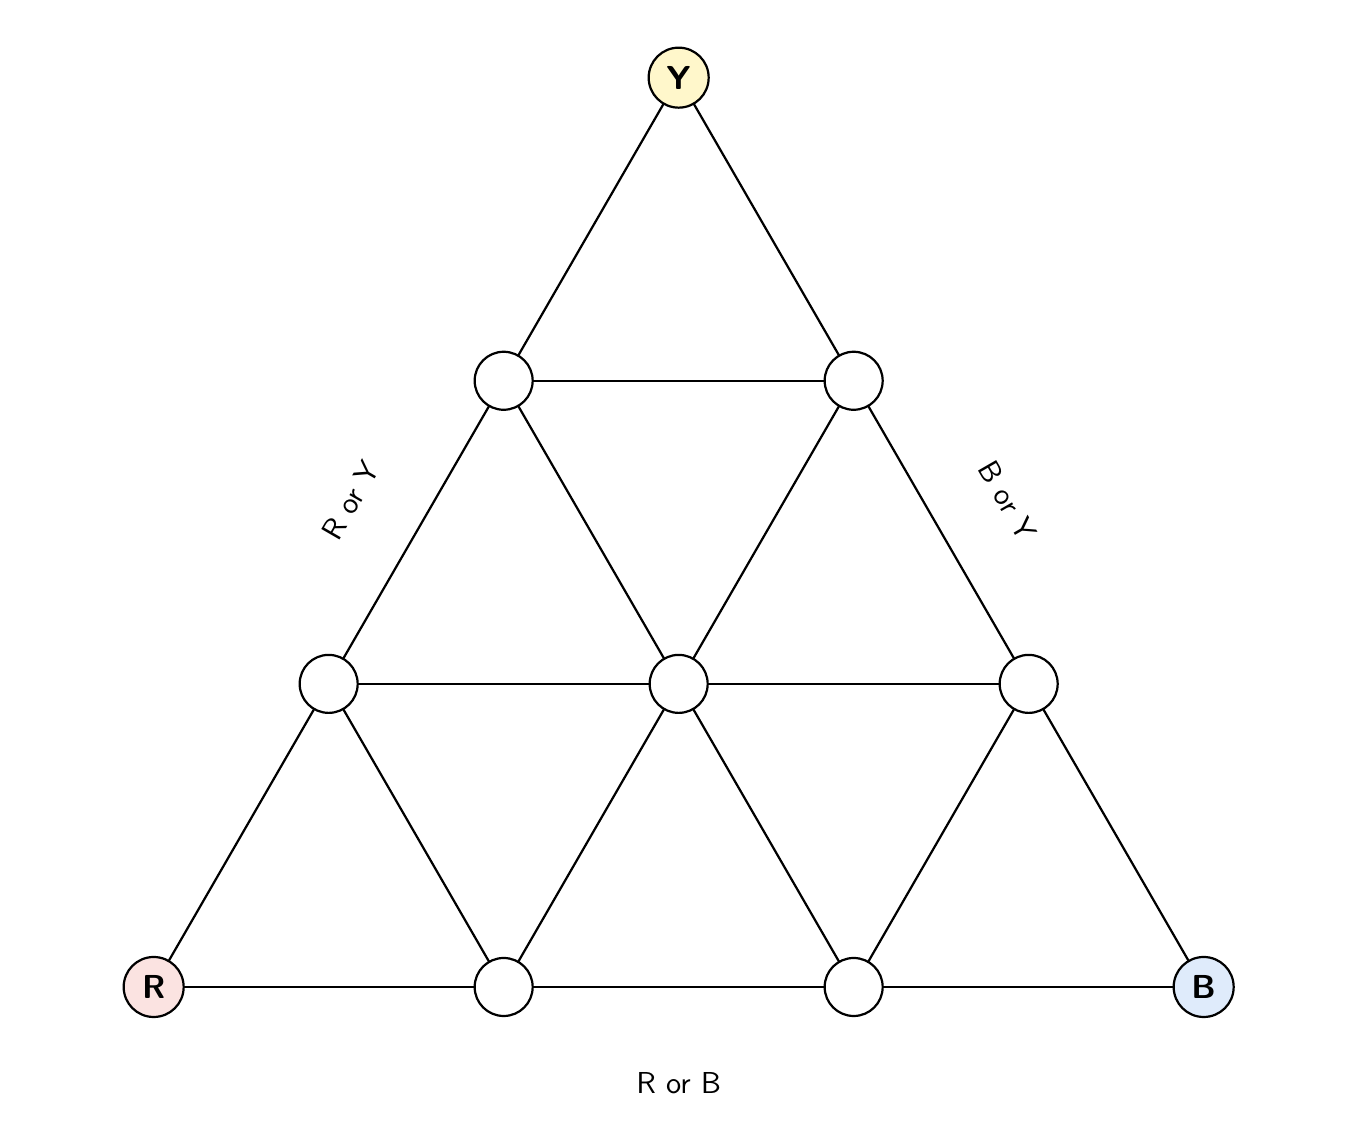
\begin{tikzpicture}[x=1in,y=1in,line cap=round,line join=round]
\path[use as bounding box] (-0.63,-0.64) rectangle (5.8800,4.7966);
\draw[line width=0.8pt] (0.0000,0.0000) -- (0.8750,1.5155);
\draw[line width=0.8pt] (0.0000,0.0000) -- (1.7500,0.0000);
\draw[line width=0.8pt] (0.8750,1.5155) -- (1.7500,3.0311);
\draw[line width=0.8pt] (0.8750,1.5155) -- (1.7500,0.0000);
\draw[line width=0.8pt] (0.8750,1.5155) -- (2.6250,1.5155);
\draw[line width=0.8pt] (1.7500,3.0311) -- (2.6250,4.5466);
\draw[line width=0.8pt] (1.7500,3.0311) -- (2.6250,1.5155);
\draw[line width=0.8pt] (1.7500,3.0311) -- (3.5000,3.0311);
\draw[line width=0.8pt] (2.6250,4.5466) -- (3.5000,3.0311);
\draw[line width=0.8pt] (1.7500,0.0000) -- (2.6250,1.5155);
\draw[line width=0.8pt] (1.7500,0.0000) -- (3.5000,0.0000);
\draw[line width=0.8pt] (2.6250,1.5155) -- (3.5000,3.0311);
\draw[line width=0.8pt] (2.6250,1.5155) -- (3.5000,0.0000);
\draw[line width=0.8pt] (2.6250,1.5155) -- (4.3750,1.5155);
\draw[line width=0.8pt] (3.5000,3.0311) -- (4.3750,1.5155);
\draw[line width=0.8pt] (3.5000,0.0000) -- (4.3750,1.5155);
\draw[line width=0.8pt] (3.5000,0.0000) -- (5.2500,0.0000);
\draw[line width=0.8pt] (4.3750,1.5155) -- (5.2500,0.0000);
\node[circle,draw,line width=0.8pt,fill=Rfill,minimum size=0.30in,inner sep=0pt,font=\sffamily\bfseries\fontsize{11.5}{12}\selectfont] at (0.0000,0.0000) {R};
\draw[line width=0.8pt,fill=white] (1.7500,0.0000) circle[radius=0.145in];
\draw[line width=0.8pt,fill=white] (3.5000,0.0000) circle[radius=0.145in];
\node[circle,draw,line width=0.8pt,fill=Bfill,minimum size=0.30in,inner sep=0pt,font=\sffamily\bfseries\fontsize{11.5}{12}\selectfont] at (5.2500,0.0000) {B};
\draw[line width=0.8pt,fill=white] (0.8750,1.5155) circle[radius=0.145in];
\draw[line width=0.8pt,fill=white] (2.6250,1.5155) circle[radius=0.145in];
\draw[line width=0.8pt,fill=white] (4.3750,1.5155) circle[radius=0.145in];
\draw[line width=0.8pt,fill=white] (1.7500,3.0311) circle[radius=0.145in];
\draw[line width=0.8pt,fill=white] (3.5000,3.0311) circle[radius=0.145in];
\node[circle,draw,line width=0.8pt,fill=Yfill,minimum size=0.30in,inner sep=0pt,font=\sffamily\bfseries\fontsize{11.5}{12}\selectfont] at (2.6250,4.5466) {Y};
\node[rotate=60,font=\sffamily\fontsize{11}{12}\selectfont] at (0.9825,2.4333) {R or Y};
\node[rotate=-60,font=\sffamily\fontsize{11}{12}\selectfont] at (4.2675,2.4333) {B or Y};
\node[font=\sffamily\fontsize{11}{12}\selectfont] at (2.6250,-0.48) {R or B};
\end{tikzpicture}
\end{center}
\newpage
\textbf{Problem 2:} An edge with R at one end and B at the other is a door. Mark every door. Draw every route that starts at an outside door. A route must leave a two-door triangle through its other door; it stops at a one-door triangle or outside. Which entrances lead back outside?\par\vspace{0.16in}
\begin{center}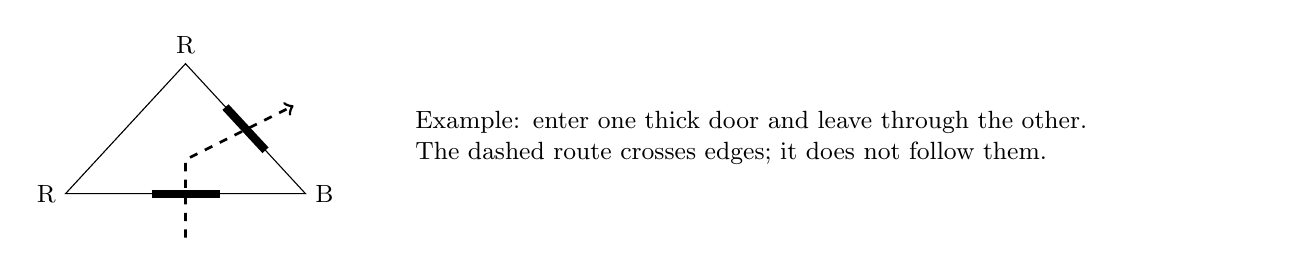
\begin{tikzpicture}[x=1in,y=1in]
\draw (0,0)--(1.2,0)--(.6,.65)--cycle;
\draw[line width=3pt] (.43,0)--(.77,0);
\draw[line width=3pt] (.80,.433)--(1.00,.217);
\node[left,font=\small] at (0,0){R};\node[right,font=\small] at (1.2,0){B};\node[above,font=\small] at (.6,.65){R};
\draw[->,dashed,line width=1pt] (.6,-.22)--(.6,.17)--(1.14,.44);
\node[anchor=west,align=left,text width=4.3in,font=\small] at (1.7,.28){Example: enter one thick door and leave through the other.\\The dashed route crosses edges; it does not follow them.};
\end{tikzpicture}\end{center}
\begin{center}
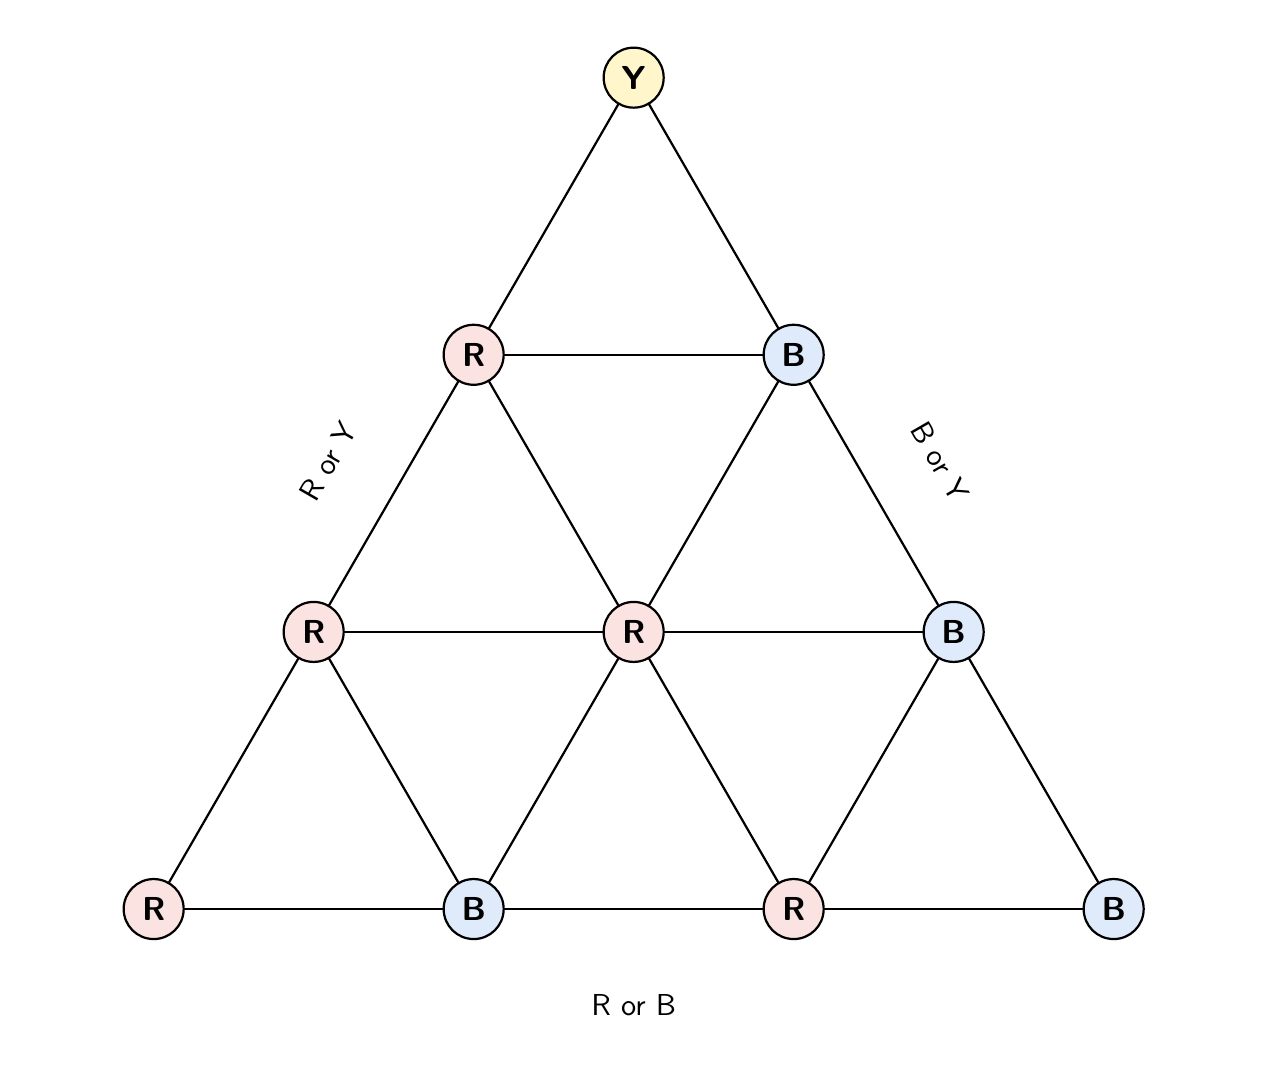
\begin{tikzpicture}[x=1in,y=1in,line cap=round,line join=round]
\path[use as bounding box] (-0.63,-0.64) rectangle (5.4300,4.4069);
\draw[line width=0.8pt] (0.0000,0.0000) -- (0.8000,1.3856);
\draw[line width=0.8pt] (0.0000,0.0000) -- (1.6000,0.0000);
\draw[line width=0.8pt] (0.8000,1.3856) -- (1.6000,2.7713);
\draw[line width=0.8pt] (0.8000,1.3856) -- (1.6000,0.0000);
\draw[line width=0.8pt] (0.8000,1.3856) -- (2.4000,1.3856);
\draw[line width=0.8pt] (1.6000,2.7713) -- (2.4000,4.1569);
\draw[line width=0.8pt] (1.6000,2.7713) -- (2.4000,1.3856);
\draw[line width=0.8pt] (1.6000,2.7713) -- (3.2000,2.7713);
\draw[line width=0.8pt] (2.4000,4.1569) -- (3.2000,2.7713);
\draw[line width=0.8pt] (1.6000,0.0000) -- (2.4000,1.3856);
\draw[line width=0.8pt] (1.6000,0.0000) -- (3.2000,0.0000);
\draw[line width=0.8pt] (2.4000,1.3856) -- (3.2000,2.7713);
\draw[line width=0.8pt] (2.4000,1.3856) -- (3.2000,0.0000);
\draw[line width=0.8pt] (2.4000,1.3856) -- (4.0000,1.3856);
\draw[line width=0.8pt] (3.2000,2.7713) -- (4.0000,1.3856);
\draw[line width=0.8pt] (3.2000,0.0000) -- (4.0000,1.3856);
\draw[line width=0.8pt] (3.2000,0.0000) -- (4.8000,0.0000);
\draw[line width=0.8pt] (4.0000,1.3856) -- (4.8000,0.0000);
\node[circle,draw,line width=0.8pt,fill=Rfill,minimum size=0.30in,inner sep=0pt,font=\sffamily\bfseries\fontsize{11.5}{12}\selectfont] at (0.0000,0.0000) {R};
\node[circle,draw,line width=0.8pt,fill=Bfill,minimum size=0.30in,inner sep=0pt,font=\sffamily\bfseries\fontsize{11.5}{12}\selectfont] at (1.6000,0.0000) {B};
\node[circle,draw,line width=0.8pt,fill=Rfill,minimum size=0.30in,inner sep=0pt,font=\sffamily\bfseries\fontsize{11.5}{12}\selectfont] at (3.2000,0.0000) {R};
\node[circle,draw,line width=0.8pt,fill=Bfill,minimum size=0.30in,inner sep=0pt,font=\sffamily\bfseries\fontsize{11.5}{12}\selectfont] at (4.8000,0.0000) {B};
\node[circle,draw,line width=0.8pt,fill=Rfill,minimum size=0.30in,inner sep=0pt,font=\sffamily\bfseries\fontsize{11.5}{12}\selectfont] at (0.8000,1.3856) {R};
\node[circle,draw,line width=0.8pt,fill=Rfill,minimum size=0.30in,inner sep=0pt,font=\sffamily\bfseries\fontsize{11.5}{12}\selectfont] at (2.4000,1.3856) {R};
\node[circle,draw,line width=0.8pt,fill=Bfill,minimum size=0.30in,inner sep=0pt,font=\sffamily\bfseries\fontsize{11.5}{12}\selectfont] at (4.0000,1.3856) {B};
\node[circle,draw,line width=0.8pt,fill=Rfill,minimum size=0.30in,inner sep=0pt,font=\sffamily\bfseries\fontsize{11.5}{12}\selectfont] at (1.6000,2.7713) {R};
\node[circle,draw,line width=0.8pt,fill=Bfill,minimum size=0.30in,inner sep=0pt,font=\sffamily\bfseries\fontsize{11.5}{12}\selectfont] at (3.2000,2.7713) {B};
\node[circle,draw,line width=0.8pt,fill=Yfill,minimum size=0.30in,inner sep=0pt,font=\sffamily\bfseries\fontsize{11.5}{12}\selectfont] at (2.4000,4.1569) {Y};
\node[rotate=60,font=\sffamily\fontsize{11}{12}\selectfont] at (0.8700,2.2385) {R or Y};
\node[rotate=-60,font=\sffamily\fontsize{11}{12}\selectfont] at (3.9300,2.2385) {B or Y};
\node[font=\sffamily\fontsize{11}{12}\selectfont] at (2.4000,-0.48) {R or B};
\end{tikzpicture}
\end{center}
\newpage
\textbf{Problem 3:} Put R, B, or Y on each dot. Find every different filling, counting turns and flips as the same. Mark the doors in each filling. Could a triangle have three doors?\par\vspace{0.16in}
\begin{center}
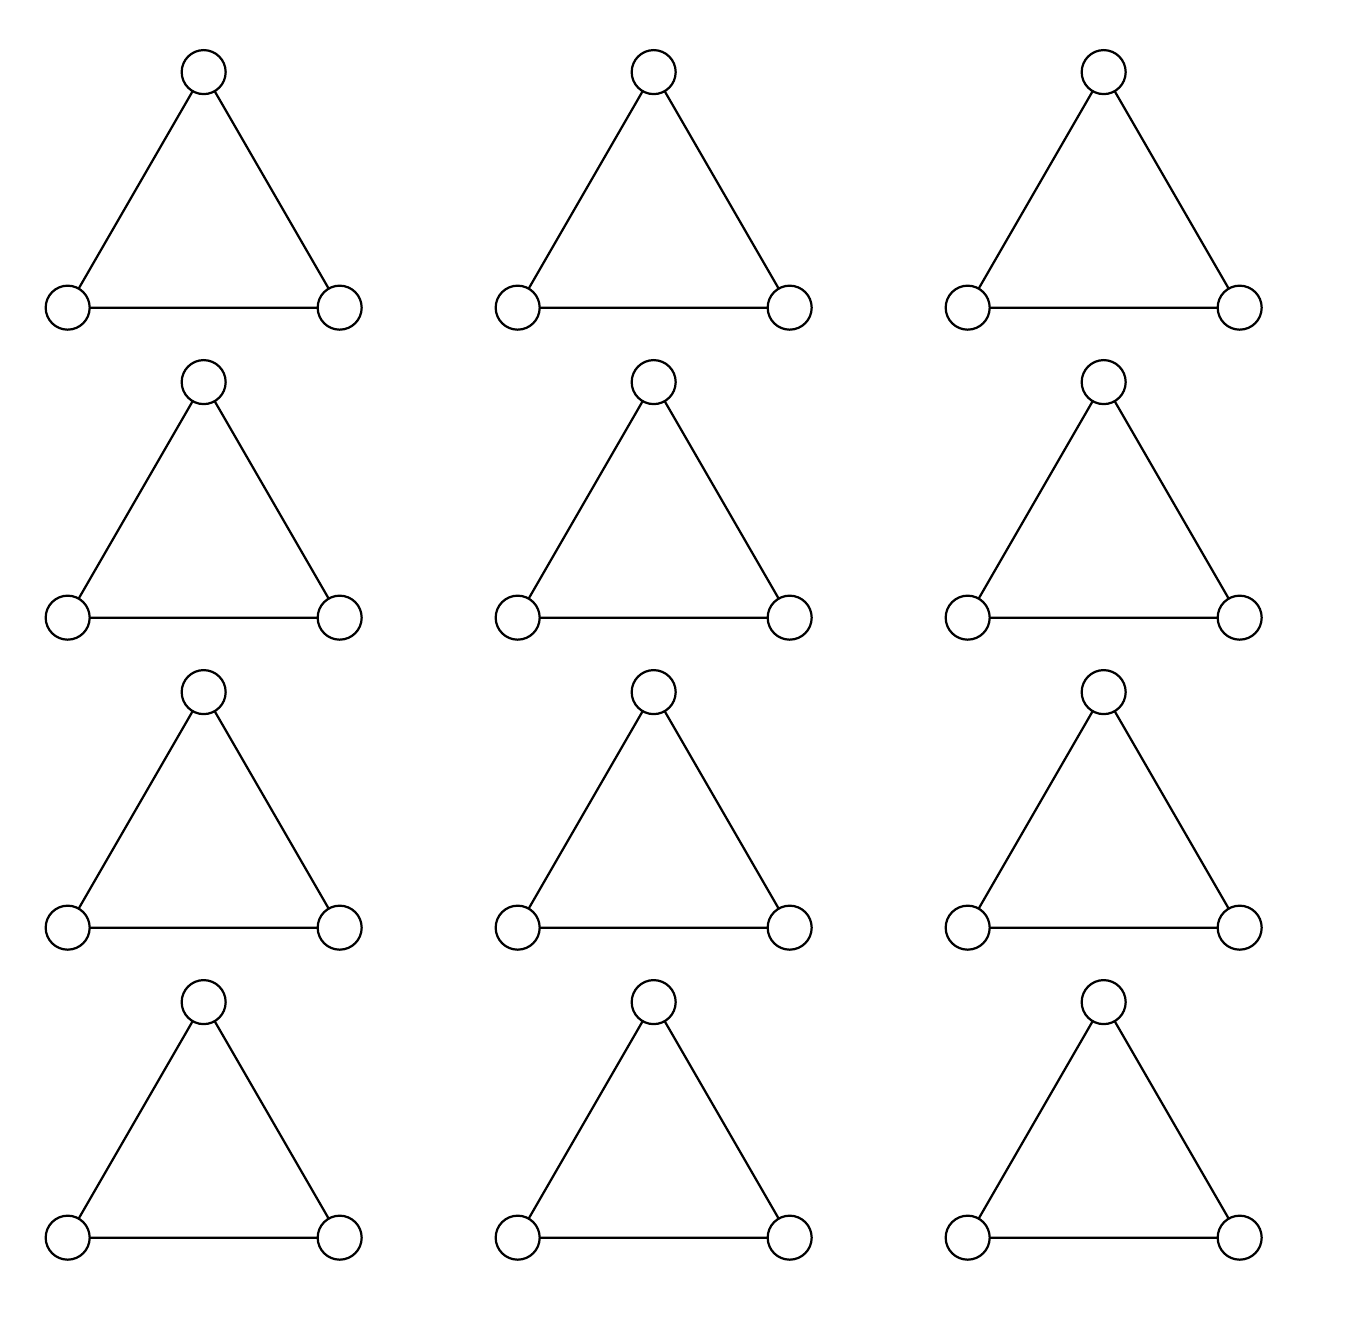
\begin{tikzpicture}[x=1in,y=1in,line cap=round]
\path[use as bounding box] (-0.2,-0.35) rectangle (6.3,6.05);
\draw[line width=0.8pt] (0.0000,4.6500) -- (1.3600,4.6500) -- (0.6800,5.8278) -- cycle;
\draw[line width=0.8pt,fill=white] (0.0000,4.6500) circle[radius=0.11in];
\draw[line width=0.8pt,fill=white] (1.3600,4.6500) circle[radius=0.11in];
\draw[line width=0.8pt,fill=white] (0.6800,5.8278) circle[radius=0.11in];
\draw[line width=0.8pt] (2.2500,4.6500) -- (3.6100,4.6500) -- (2.9300,5.8278) -- cycle;
\draw[line width=0.8pt,fill=white] (2.2500,4.6500) circle[radius=0.11in];
\draw[line width=0.8pt,fill=white] (3.6100,4.6500) circle[radius=0.11in];
\draw[line width=0.8pt,fill=white] (2.9300,5.8278) circle[radius=0.11in];
\draw[line width=0.8pt] (4.5000,4.6500) -- (5.8600,4.6500) -- (5.1800,5.8278) -- cycle;
\draw[line width=0.8pt,fill=white] (4.5000,4.6500) circle[radius=0.11in];
\draw[line width=0.8pt,fill=white] (5.8600,4.6500) circle[radius=0.11in];
\draw[line width=0.8pt,fill=white] (5.1800,5.8278) circle[radius=0.11in];
\draw[line width=0.8pt] (0.0000,3.1000) -- (1.3600,3.1000) -- (0.6800,4.2778) -- cycle;
\draw[line width=0.8pt,fill=white] (0.0000,3.1000) circle[radius=0.11in];
\draw[line width=0.8pt,fill=white] (1.3600,3.1000) circle[radius=0.11in];
\draw[line width=0.8pt,fill=white] (0.6800,4.2778) circle[radius=0.11in];
\draw[line width=0.8pt] (2.2500,3.1000) -- (3.6100,3.1000) -- (2.9300,4.2778) -- cycle;
\draw[line width=0.8pt,fill=white] (2.2500,3.1000) circle[radius=0.11in];
\draw[line width=0.8pt,fill=white] (3.6100,3.1000) circle[radius=0.11in];
\draw[line width=0.8pt,fill=white] (2.9300,4.2778) circle[radius=0.11in];
\draw[line width=0.8pt] (4.5000,3.1000) -- (5.8600,3.1000) -- (5.1800,4.2778) -- cycle;
\draw[line width=0.8pt,fill=white] (4.5000,3.1000) circle[radius=0.11in];
\draw[line width=0.8pt,fill=white] (5.8600,3.1000) circle[radius=0.11in];
\draw[line width=0.8pt,fill=white] (5.1800,4.2778) circle[radius=0.11in];
\draw[line width=0.8pt] (0.0000,1.5500) -- (1.3600,1.5500) -- (0.6800,2.7278) -- cycle;
\draw[line width=0.8pt,fill=white] (0.0000,1.5500) circle[radius=0.11in];
\draw[line width=0.8pt,fill=white] (1.3600,1.5500) circle[radius=0.11in];
\draw[line width=0.8pt,fill=white] (0.6800,2.7278) circle[radius=0.11in];
\draw[line width=0.8pt] (2.2500,1.5500) -- (3.6100,1.5500) -- (2.9300,2.7278) -- cycle;
\draw[line width=0.8pt,fill=white] (2.2500,1.5500) circle[radius=0.11in];
\draw[line width=0.8pt,fill=white] (3.6100,1.5500) circle[radius=0.11in];
\draw[line width=0.8pt,fill=white] (2.9300,2.7278) circle[radius=0.11in];
\draw[line width=0.8pt] (4.5000,1.5500) -- (5.8600,1.5500) -- (5.1800,2.7278) -- cycle;
\draw[line width=0.8pt,fill=white] (4.5000,1.5500) circle[radius=0.11in];
\draw[line width=0.8pt,fill=white] (5.8600,1.5500) circle[radius=0.11in];
\draw[line width=0.8pt,fill=white] (5.1800,2.7278) circle[radius=0.11in];
\draw[line width=0.8pt] (0.0000,0.0000) -- (1.3600,0.0000) -- (0.6800,1.1778) -- cycle;
\draw[line width=0.8pt,fill=white] (0.0000,0.0000) circle[radius=0.11in];
\draw[line width=0.8pt,fill=white] (1.3600,0.0000) circle[radius=0.11in];
\draw[line width=0.8pt,fill=white] (0.6800,1.1778) circle[radius=0.11in];
\draw[line width=0.8pt] (2.2500,0.0000) -- (3.6100,0.0000) -- (2.9300,1.1778) -- cycle;
\draw[line width=0.8pt,fill=white] (2.2500,0.0000) circle[radius=0.11in];
\draw[line width=0.8pt,fill=white] (3.6100,0.0000) circle[radius=0.11in];
\draw[line width=0.8pt,fill=white] (2.9300,1.1778) circle[radius=0.11in];
\draw[line width=0.8pt] (4.5000,0.0000) -- (5.8600,0.0000) -- (5.1800,1.1778) -- cycle;
\draw[line width=0.8pt,fill=white] (4.5000,0.0000) circle[radius=0.11in];
\draw[line width=0.8pt,fill=white] (5.8600,0.0000) circle[radius=0.11in];
\draw[line width=0.8pt,fill=white] (5.1800,1.1778) circle[radius=0.11in];
\end{tikzpicture}
\end{center}
\newpage
\textbf{Problem 4:} Write R or B on every empty dot and mark the doors. Can any row have an even number of doors? Explain why or why not.\par\vspace{0.16in}
\begin{center}
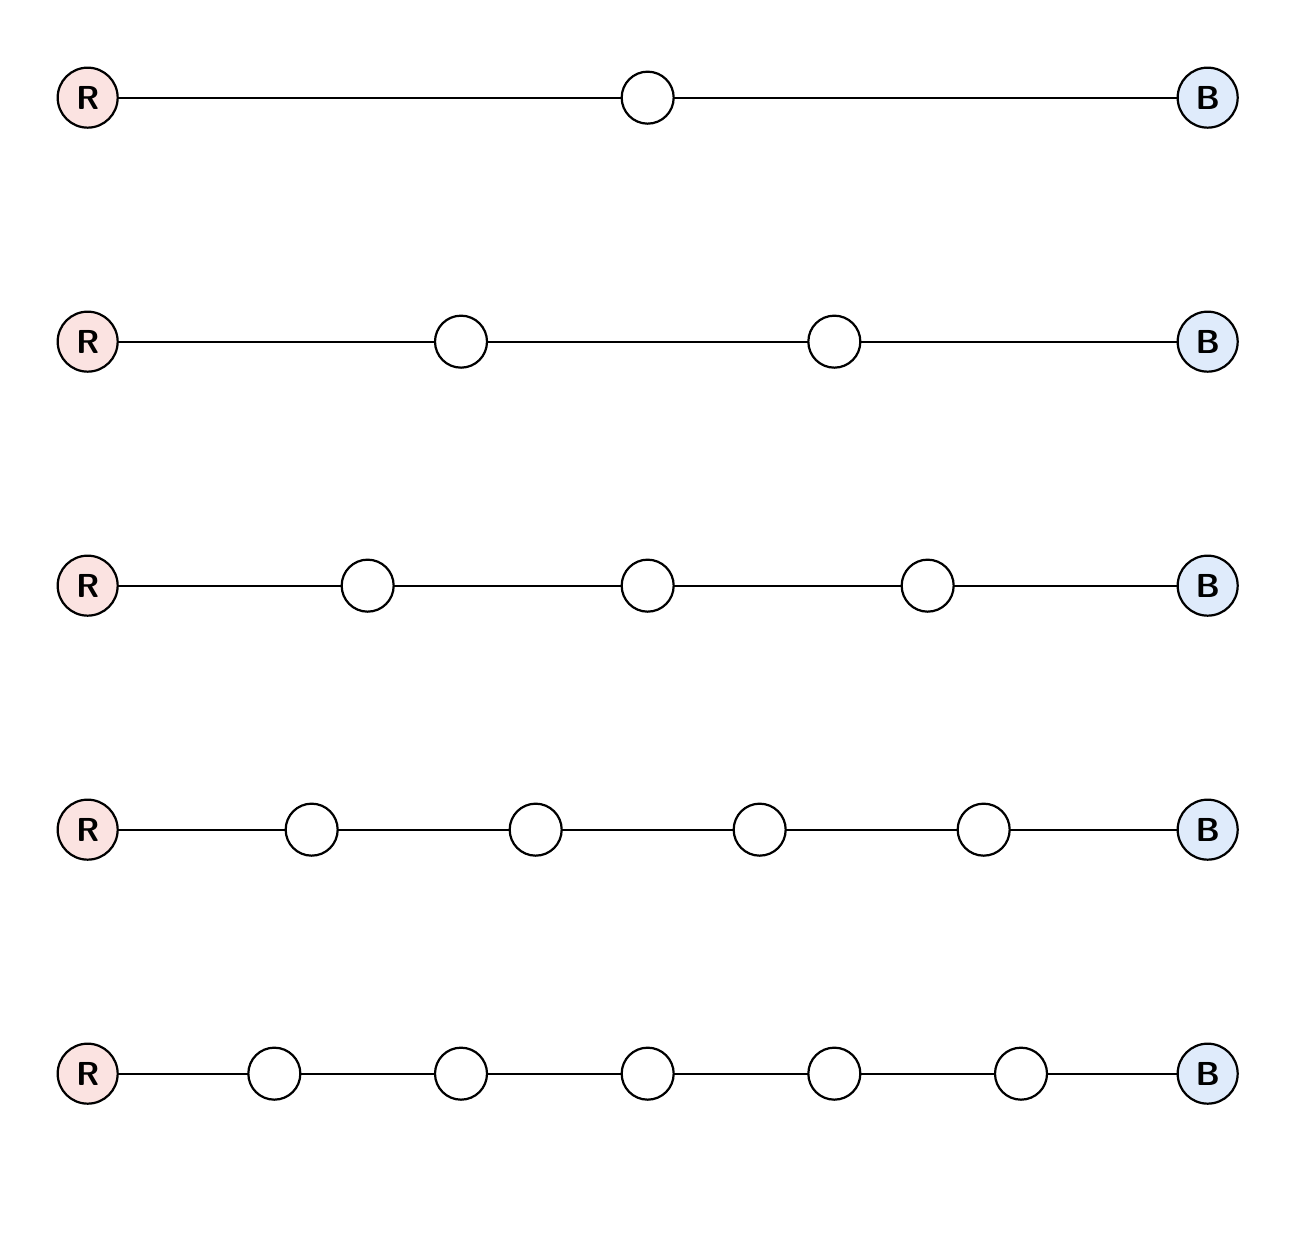
\begin{tikzpicture}[x=1in,y=1in,line cap=round]
\path[use as bounding box] (-0.3,-0.25) rectangle (5.9,5.65);
\draw[line width=0.8pt] (0,5.3000) -- (5.6,5.3000);
\node[circle,draw,line width=0.8pt,fill=Rfill,minimum size=0.30in,inner sep=0pt,font=\sffamily\bfseries\fontsize{11.5}{12}\selectfont] at (0.0000,5.3000) {R};
\draw[line width=0.8pt,fill=white] (2.8000,5.3000) circle[radius=0.13in];
\node[circle,draw,line width=0.8pt,fill=Bfill,minimum size=0.30in,inner sep=0pt,font=\sffamily\bfseries\fontsize{11.5}{12}\selectfont] at (5.6000,5.3000) {B};
\draw[line width=0.8pt] (0,4.0800) -- (5.6,4.0800);
\node[circle,draw,line width=0.8pt,fill=Rfill,minimum size=0.30in,inner sep=0pt,font=\sffamily\bfseries\fontsize{11.5}{12}\selectfont] at (0.0000,4.0800) {R};
\draw[line width=0.8pt,fill=white] (1.8667,4.0800) circle[radius=0.13in];
\draw[line width=0.8pt,fill=white] (3.7333,4.0800) circle[radius=0.13in];
\node[circle,draw,line width=0.8pt,fill=Bfill,minimum size=0.30in,inner sep=0pt,font=\sffamily\bfseries\fontsize{11.5}{12}\selectfont] at (5.6000,4.0800) {B};
\draw[line width=0.8pt] (0,2.8600) -- (5.6,2.8600);
\node[circle,draw,line width=0.8pt,fill=Rfill,minimum size=0.30in,inner sep=0pt,font=\sffamily\bfseries\fontsize{11.5}{12}\selectfont] at (0.0000,2.8600) {R};
\draw[line width=0.8pt,fill=white] (1.4000,2.8600) circle[radius=0.13in];
\draw[line width=0.8pt,fill=white] (2.8000,2.8600) circle[radius=0.13in];
\draw[line width=0.8pt,fill=white] (4.2000,2.8600) circle[radius=0.13in];
\node[circle,draw,line width=0.8pt,fill=Bfill,minimum size=0.30in,inner sep=0pt,font=\sffamily\bfseries\fontsize{11.5}{12}\selectfont] at (5.6000,2.8600) {B};
\draw[line width=0.8pt] (0,1.6400) -- (5.6,1.6400);
\node[circle,draw,line width=0.8pt,fill=Rfill,minimum size=0.30in,inner sep=0pt,font=\sffamily\bfseries\fontsize{11.5}{12}\selectfont] at (0.0000,1.6400) {R};
\draw[line width=0.8pt,fill=white] (1.1200,1.6400) circle[radius=0.13in];
\draw[line width=0.8pt,fill=white] (2.2400,1.6400) circle[radius=0.13in];
\draw[line width=0.8pt,fill=white] (3.3600,1.6400) circle[radius=0.13in];
\draw[line width=0.8pt,fill=white] (4.4800,1.6400) circle[radius=0.13in];
\node[circle,draw,line width=0.8pt,fill=Bfill,minimum size=0.30in,inner sep=0pt,font=\sffamily\bfseries\fontsize{11.5}{12}\selectfont] at (5.6000,1.6400) {B};
\draw[line width=0.8pt] (0,0.4200) -- (5.6,0.4200);
\node[circle,draw,line width=0.8pt,fill=Rfill,minimum size=0.30in,inner sep=0pt,font=\sffamily\bfseries\fontsize{11.5}{12}\selectfont] at (0.0000,0.4200) {R};
\draw[line width=0.8pt,fill=white] (0.9333,0.4200) circle[radius=0.13in];
\draw[line width=0.8pt,fill=white] (1.8667,0.4200) circle[radius=0.13in];
\draw[line width=0.8pt,fill=white] (2.8000,0.4200) circle[radius=0.13in];
\draw[line width=0.8pt,fill=white] (3.7333,0.4200) circle[radius=0.13in];
\draw[line width=0.8pt,fill=white] (4.6667,0.4200) circle[radius=0.13in];
\node[circle,draw,line width=0.8pt,fill=Bfill,minimum size=0.30in,inner sep=0pt,font=\sffamily\bfseries\fontsize{11.5}{12}\selectfont] at (5.6000,0.4200) {B};
\end{tikzpicture}
\end{center}
\newpage
\textbf{Problem 5:} Fill the dots so that exactly three little triangles have R, B, and Y. Draw all routes that start at outside doors. Can all those routes end outside?\par\vspace{0.16in}
\begin{center}
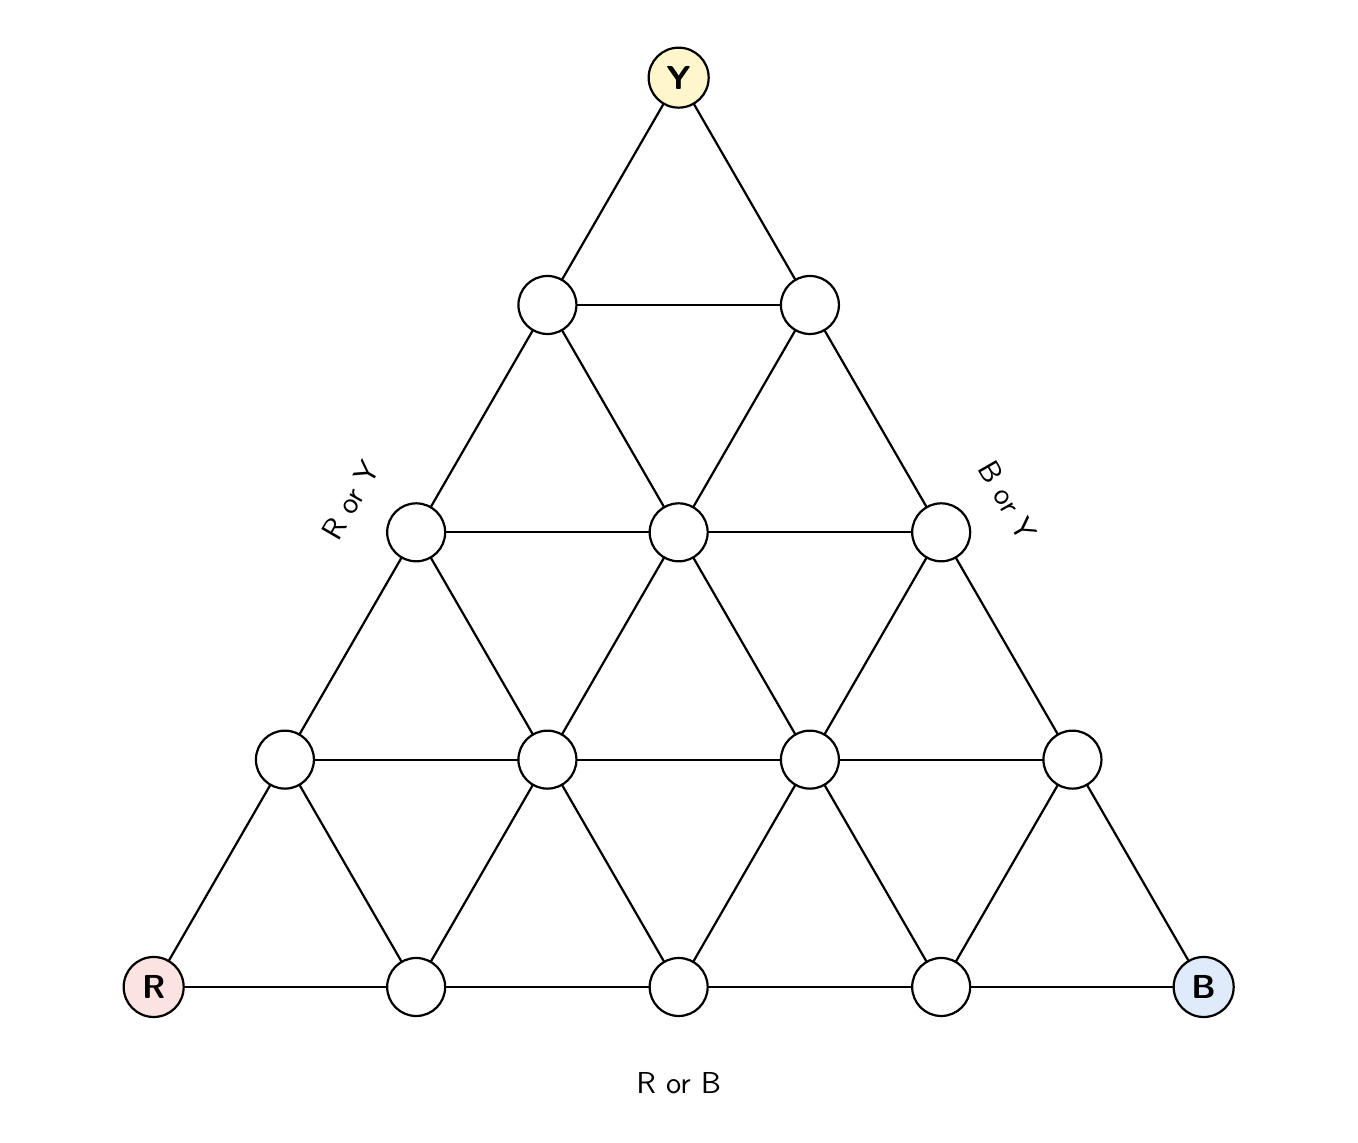
\begin{tikzpicture}[x=1in,y=1in,line cap=round,line join=round]
\path[use as bounding box] (-0.63,-0.64) rectangle (5.8800,4.7966);
\draw[line width=0.8pt] (0.0000,0.0000) -- (0.6562,1.1367);
\draw[line width=0.8pt] (0.0000,0.0000) -- (1.3125,0.0000);
\draw[line width=0.8pt] (0.6562,1.1367) -- (1.3125,2.2733);
\draw[line width=0.8pt] (0.6562,1.1367) -- (1.3125,0.0000);
\draw[line width=0.8pt] (0.6562,1.1367) -- (1.9688,1.1367);
\draw[line width=0.8pt] (1.3125,2.2733) -- (1.9688,3.4100);
\draw[line width=0.8pt] (1.3125,2.2733) -- (1.9688,1.1367);
\draw[line width=0.8pt] (1.3125,2.2733) -- (2.6250,2.2733);
\draw[line width=0.8pt] (1.9688,3.4100) -- (2.6250,4.5466);
\draw[line width=0.8pt] (1.9688,3.4100) -- (2.6250,2.2733);
\draw[line width=0.8pt] (1.9688,3.4100) -- (3.2812,3.4100);
\draw[line width=0.8pt] (2.6250,4.5466) -- (3.2812,3.4100);
\draw[line width=0.8pt] (1.3125,0.0000) -- (1.9688,1.1367);
\draw[line width=0.8pt] (1.3125,0.0000) -- (2.6250,0.0000);
\draw[line width=0.8pt] (1.9688,1.1367) -- (2.6250,2.2733);
\draw[line width=0.8pt] (1.9688,1.1367) -- (2.6250,0.0000);
\draw[line width=0.8pt] (1.9688,1.1367) -- (3.2812,1.1367);
\draw[line width=0.8pt] (2.6250,2.2733) -- (3.2812,3.4100);
\draw[line width=0.8pt] (2.6250,2.2733) -- (3.2812,1.1367);
\draw[line width=0.8pt] (2.6250,2.2733) -- (3.9375,2.2733);
\draw[line width=0.8pt] (3.2812,3.4100) -- (3.9375,2.2733);
\draw[line width=0.8pt] (2.6250,0.0000) -- (3.2812,1.1367);
\draw[line width=0.8pt] (2.6250,0.0000) -- (3.9375,0.0000);
\draw[line width=0.8pt] (3.2812,1.1367) -- (3.9375,2.2733);
\draw[line width=0.8pt] (3.2812,1.1367) -- (3.9375,0.0000);
\draw[line width=0.8pt] (3.2812,1.1367) -- (4.5938,1.1367);
\draw[line width=0.8pt] (3.9375,2.2733) -- (4.5938,1.1367);
\draw[line width=0.8pt] (3.9375,0.0000) -- (4.5938,1.1367);
\draw[line width=0.8pt] (3.9375,0.0000) -- (5.2500,0.0000);
\draw[line width=0.8pt] (4.5938,1.1367) -- (5.2500,0.0000);
\node[circle,draw,line width=0.8pt,fill=Rfill,minimum size=0.30in,inner sep=0pt,font=\sffamily\bfseries\fontsize{11.5}{12}\selectfont] at (0.0000,0.0000) {R};
\draw[line width=0.8pt,fill=white] (1.3125,0.0000) circle[radius=0.145in];
\draw[line width=0.8pt,fill=white] (2.6250,0.0000) circle[radius=0.145in];
\draw[line width=0.8pt,fill=white] (3.9375,0.0000) circle[radius=0.145in];
\node[circle,draw,line width=0.8pt,fill=Bfill,minimum size=0.30in,inner sep=0pt,font=\sffamily\bfseries\fontsize{11.5}{12}\selectfont] at (5.2500,0.0000) {B};
\draw[line width=0.8pt,fill=white] (0.6562,1.1367) circle[radius=0.145in];
\draw[line width=0.8pt,fill=white] (1.9688,1.1367) circle[radius=0.145in];
\draw[line width=0.8pt,fill=white] (3.2812,1.1367) circle[radius=0.145in];
\draw[line width=0.8pt,fill=white] (4.5938,1.1367) circle[radius=0.145in];
\draw[line width=0.8pt,fill=white] (1.3125,2.2733) circle[radius=0.145in];
\draw[line width=0.8pt,fill=white] (2.6250,2.2733) circle[radius=0.145in];
\draw[line width=0.8pt,fill=white] (3.9375,2.2733) circle[radius=0.145in];
\draw[line width=0.8pt,fill=white] (1.9688,3.4100) circle[radius=0.145in];
\draw[line width=0.8pt,fill=white] (3.2812,3.4100) circle[radius=0.145in];
\node[circle,draw,line width=0.8pt,fill=Yfill,minimum size=0.30in,inner sep=0pt,font=\sffamily\bfseries\fontsize{11.5}{12}\selectfont] at (2.6250,4.5466) {Y};
\node[rotate=60,font=\sffamily\fontsize{11}{12}\selectfont] at (0.9825,2.4333) {R or Y};
\node[rotate=-60,font=\sffamily\fontsize{11}{12}\selectfont] at (4.2675,2.4333) {B or Y};
\node[font=\sffamily\fontsize{11}{12}\selectfont] at (2.6250,-0.48) {R or B};
\end{tikzpicture}
\end{center}
\newpage
\textbf{Problem 6:} Can the dots be filled so that no little triangle has R, B, and Y? Give a reason that covers every filling allowed by the side rules.\par\vspace{0.16in}
\begin{center}
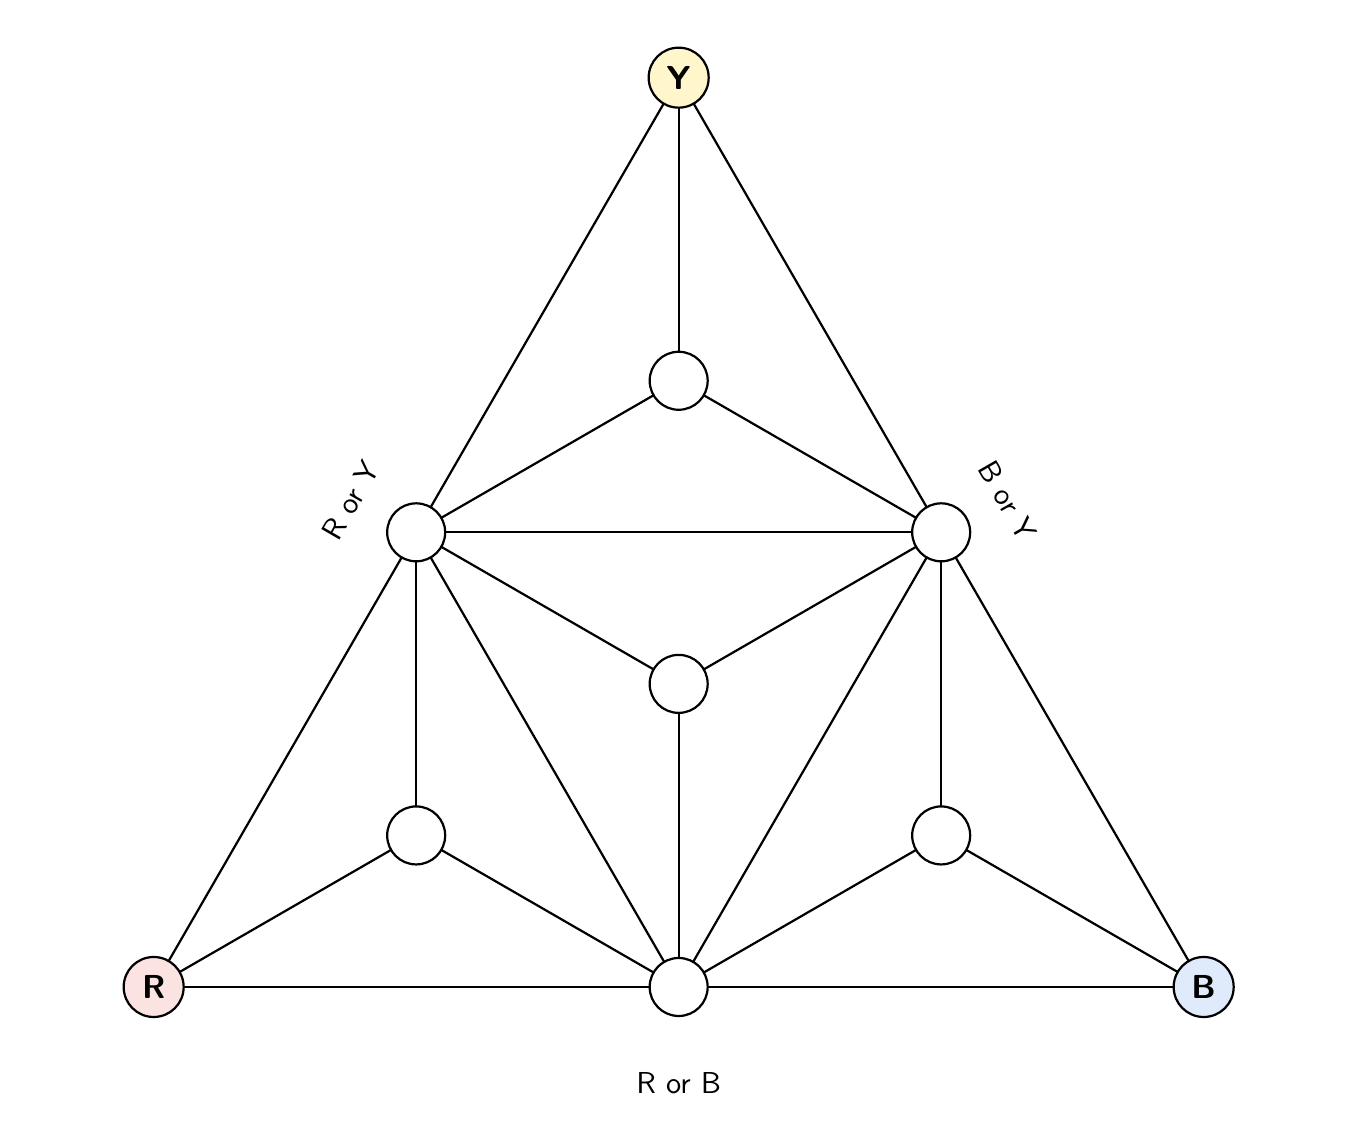
\begin{tikzpicture}[x=1in,y=1in,line cap=round,line join=round]
\path[use as bounding box] (-0.63,-0.64) rectangle (5.8800,4.7966);
\draw[line width=0.8pt] (0.0000,0.0000) -- (1.3125,2.2733);
\draw[line width=0.8pt] (0.0000,0.0000) -- (2.6250,0.0000);
\draw[line width=0.8pt] (0.0000,0.0000) -- (1.3125,0.7578);
\draw[line width=0.8pt] (1.3125,2.2733) -- (2.6250,4.5466);
\draw[line width=0.8pt] (1.3125,2.2733) -- (2.6250,0.0000);
\draw[line width=0.8pt] (1.3125,2.2733) -- (3.9375,2.2733);
\draw[line width=0.8pt] (1.3125,2.2733) -- (1.3125,0.7578);
\draw[line width=0.8pt] (1.3125,2.2733) -- (2.6250,1.5155);
\draw[line width=0.8pt] (1.3125,2.2733) -- (2.6250,3.0311);
\draw[line width=0.8pt] (2.6250,4.5466) -- (3.9375,2.2733);
\draw[line width=0.8pt] (2.6250,4.5466) -- (2.6250,3.0311);
\draw[line width=0.8pt] (2.6250,0.0000) -- (3.9375,2.2733);
\draw[line width=0.8pt] (2.6250,0.0000) -- (5.2500,0.0000);
\draw[line width=0.8pt] (2.6250,0.0000) -- (1.3125,0.7578);
\draw[line width=0.8pt] (2.6250,0.0000) -- (2.6250,1.5155);
\draw[line width=0.8pt] (2.6250,0.0000) -- (3.9375,0.7578);
\draw[line width=0.8pt] (3.9375,2.2733) -- (5.2500,0.0000);
\draw[line width=0.8pt] (3.9375,2.2733) -- (2.6250,1.5155);
\draw[line width=0.8pt] (3.9375,2.2733) -- (3.9375,0.7578);
\draw[line width=0.8pt] (3.9375,2.2733) -- (2.6250,3.0311);
\draw[line width=0.8pt] (5.2500,0.0000) -- (3.9375,0.7578);
\node[circle,draw,line width=0.8pt,fill=Rfill,minimum size=0.30in,inner sep=0pt,font=\sffamily\bfseries\fontsize{11.5}{12}\selectfont] at (0.0000,0.0000) {R};
\draw[line width=0.8pt,fill=white] (2.6250,0.0000) circle[radius=0.145in];
\node[circle,draw,line width=0.8pt,fill=Bfill,minimum size=0.30in,inner sep=0pt,font=\sffamily\bfseries\fontsize{11.5}{12}\selectfont] at (5.2500,0.0000) {B};
\draw[line width=0.8pt,fill=white] (1.3125,2.2733) circle[radius=0.145in];
\draw[line width=0.8pt,fill=white] (3.9375,2.2733) circle[radius=0.145in];
\node[circle,draw,line width=0.8pt,fill=Yfill,minimum size=0.30in,inner sep=0pt,font=\sffamily\bfseries\fontsize{11.5}{12}\selectfont] at (2.6250,4.5466) {Y};
\draw[line width=0.8pt,fill=white] (1.3125,0.7578) circle[radius=0.145in];
\draw[line width=0.8pt,fill=white] (2.6250,1.5155) circle[radius=0.145in];
\draw[line width=0.8pt,fill=white] (3.9375,0.7578) circle[radius=0.145in];
\draw[line width=0.8pt,fill=white] (2.6250,3.0311) circle[radius=0.145in];
\node[rotate=60,font=\sffamily\fontsize{11}{12}\selectfont] at (0.9825,2.4333) {R or Y};
\node[rotate=-60,font=\sffamily\fontsize{11}{12}\selectfont] at (4.2675,2.4333) {B or Y};
\node[font=\sffamily\fontsize{11}{12}\selectfont] at (2.6250,-0.48) {R or B};
\end{tikzpicture}
\end{center}
\end{document}
